Rewriting the given lines as 
\begin{align}
 L_1: \frac{x - 1}{-3}=\frac{y-2}{\frac{2}{7}p}=\frac{z-3}{2}
\\
 L_2: \frac{x - 1}{\frac{-3}{7}p}=\frac{y-5}{1}=\frac{z-6}{-5}
 \end{align}
 Using the definition of a line in co-ordinate geometry, we see from the above two equations, the direction vectors \textbf{a} and \textbf{b} of the two lines are
 \begin{align}
 \vec{a} = 
 \myvec{-3\\
  \frac{2}{7}p\\
  2}
\\
  \vec{b} = 
 \myvec{\frac{-3}{7}p\\
  1\\
  -5}
 \end{align}
 respectively.\\
 In order for the two lines to be perpendicular, their dot product should be equal to 0 which gives,
 \begin{equation}
 \frac{\vec{a}^T\vec{b}}{\norm{\textbf{a}}\norm{\textbf{b}}} = 0
 \end{equation}
 Which in turn gives us,
 \begin{align}
 \vec{a}^T\vec{b} = \frac{11}{7}p - 10
 \\
 \implies \frac{11}{7}p - 10 = 0
 \\  
 \implies p = \frac{70}{11} 
 \\
 \implies p \approx 6.364
 \end{align}
See Fig.   \ref{fig:solutions/line_plane/75/Figures}

 \begin{figure}[h]
 \centering
 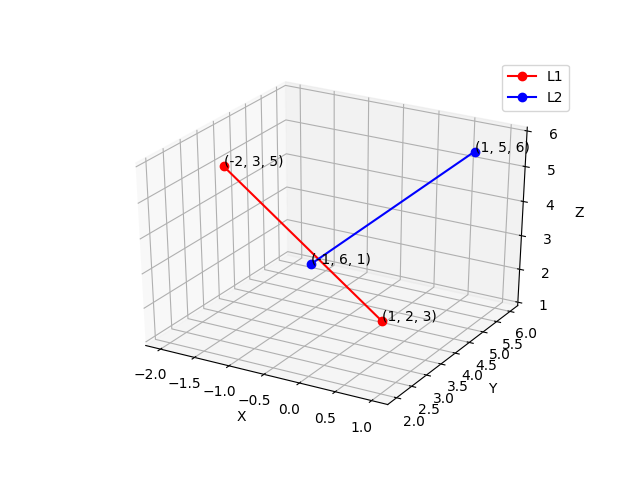
\includegraphics[width=\columnwidth]{./solutions/line_plane/75/Figures/lines.png}
 \caption{The two lines plotted by substituting the value of $p$ found}
 \label{fig:solutions/line_plane/75/Figures}
 \end{figure}
